\documentclass[12pt, a4 paper]{article}
\usepackage{geometry}
\geometry{left=2cm, right=2cm, top=1.5cm, bottom=1.5cm}
\usepackage{amsmath}
\usepackage{amssymb}
\usepackage{amsfonts}
\usepackage{framed}
\usepackage{caption}
\usepackage{indentfirst}
\usepackage{graphicx}
\setlength{\parskip}{0.5em}
\title{Homography Matrix Estimation}
\author{\textup{Xueren Ge}}

\begin{document}



\begin{titlepage}
	\newcommand{\HRule}{\rule{\linewidth}{0.5mm}}
	\center 
	\quad\\[1.5cm]
	\textsl{\Large Georgia Institute of Technology }\\[0.5cm] 
	\textsl{\large School of Electrical and Computer Engineering}\\[0.5cm] 
	\makeatletter
	\HRule \\[0.4cm]
	{ \huge \bfseries \@title}\\[0.4cm] 
	\HRule \\[1.5cm]
	\begin{minipage}{0.4\textwidth}
		\begin{flushleft} \large
			\emph{Author:}\\
			\@author
		\end{flushleft}
    \end{minipage}
    ~
	\begin{minipage}{0.4\textwidth}
		\begin{flushright} \large
			\emph{Supervisor:} \\
			\textup{Nope}
		\end{flushright}
	\end{minipage}\\[3cm]
	\makeatother
	{\large Robot}\\[0.5cm]
	{\large \today}\\[2cm] 
	\vfill 
\end{titlepage}


\section{Graph Transformation}
\subsection{Rotation}
If you rotate a picture around origin $(0, 0)$
counterclockwise by $\theta$ agnle, we can have,
\begin{figure}[h]
    \centering
    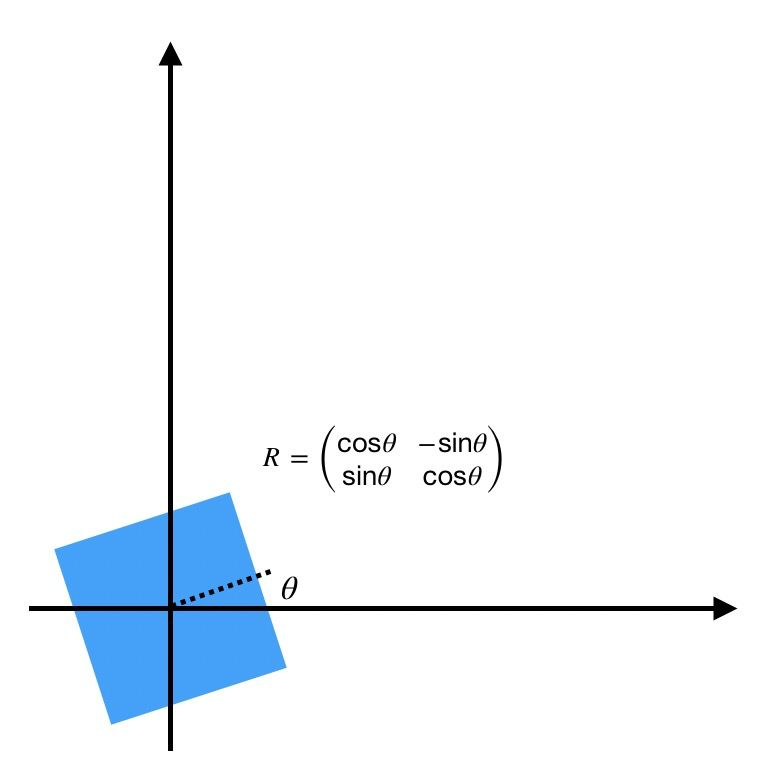
\includegraphics[width=10cm,height=9cm]{rotation.jpg}
    \caption{rotation}
\end{figure}

\begin{align}
    x^{\prime} &= x \cdot \cos\theta - y \cdot \sin\theta\\
    y^{\prime} &= x \cdot \sin\theta + y \cdot \cos\theta
\end{align}
\indent written in the form of matrix multiplication,
\begin{equation}
    \begin{pmatrix} x^{\prime} \\ y^{\prime} \end{pmatrix}=
    \begin{bmatrix} \cos\theta & -\sin\theta
    \\ \sin\theta & \cos\theta \end{bmatrix}
    \begin{pmatrix} x \\ y \end{pmatrix}
\end{equation}

\subsection{Translation}
Translation can be described as,
\begin{align}
    x^{\prime} &= x + t_{x}\\
    y^{\prime} &= y + t_{y}
\end{align}
\indent In matrix form, we have
\begin{equation}
    \begin{pmatrix} x^{\prime} \\ y^{\prime} \end{pmatrix}=
    \begin{pmatrix} x \\ y \end{pmatrix} + 
    \begin{bmatrix} t_{x} \\ t_{y} \end{bmatrix}
\end{equation}
\begin{figure}[h]
    \centering
    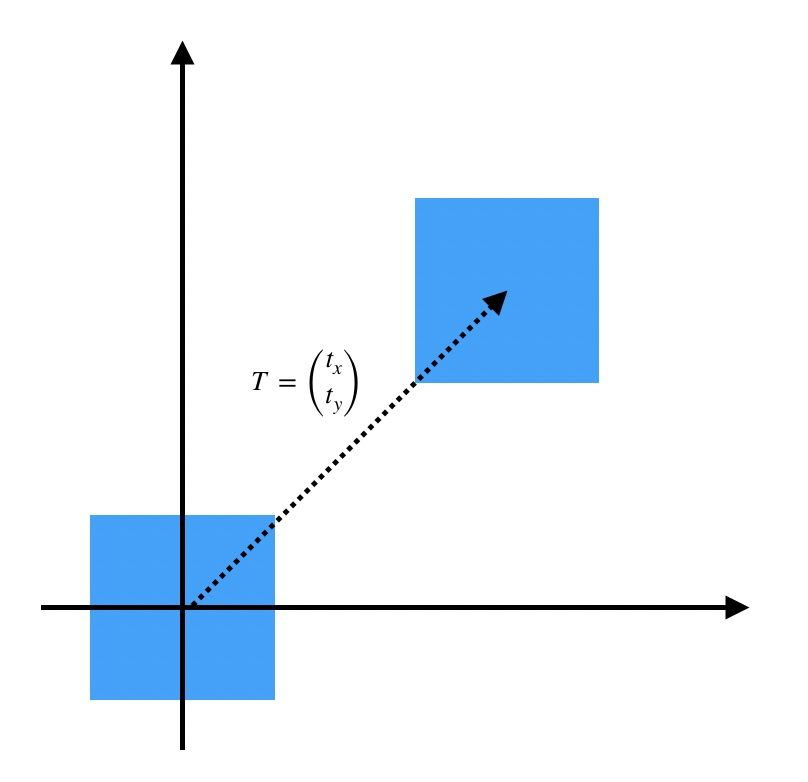
\includegraphics[width=10cm,height=9cm]{translation.jpg}
    \caption{translation}
\end{figure}
\indent Here comes the problem, that is we can't write it as
matrix multiplication form. To solve this problem, let's 
introduce homogeneous coordinate system, where $(x, y )
\iff (x, y ,1)$, and then write it as matrix multiplication,
\begin{equation}
    \begin{pmatrix}
        x^{\prime} \\ y^{\prime} \\ 1
    \end{pmatrix} = 
    \begin{bmatrix}
        1 & 0 & t_{x} \\ 0 & 1 & t_{y} \\ 0 & 0 & 1
    \end{bmatrix} 
    \begin{pmatrix}
        x \\ y \\ 1
    \end{pmatrix} = 
    \begin{bmatrix}
        \boldsymbol{I}_{2 \times 2} & \boldsymbol{T}_{2 \times 1}\\
        \boldsymbol{0}^{T} & \boldsymbol{1}
    \end{bmatrix}
    \begin{pmatrix}
        x \\ y \\ 1
    \end{pmatrix}
\end{equation}
\indent and then, we can combine rotation with translation, which
is \textbf{Rigid Body Transformation},
\begin{equation}
    \begin{pmatrix}
        x^{\prime} \\ y^{\prime} \\ 1
    \end{pmatrix} = 
    \begin{bmatrix}
        \cos\theta & -\sin\theta & t_{x} \\
        \sin\theta & \cos\theta & t_{y} \\
         0 & 0 & 1
    \end{bmatrix} 
    \begin{pmatrix}
        x \\ y \\ 1
    \end{pmatrix} = 
    \begin{bmatrix}
        \boldsymbol{R}_{2 \times 2} & \boldsymbol{T}_{2 \times 1}\\
        \boldsymbol{0}^{T} & \boldsymbol{1}
    \end{bmatrix}
    \begin{pmatrix}
        x \\ y \\ 1
    \end{pmatrix}
\end{equation}
\indent Note that here rotation matrix $\boldsymbol{R}_{2\times 2}$
is orthogonal matrix.
\begin{figure}[h]
    \centering
    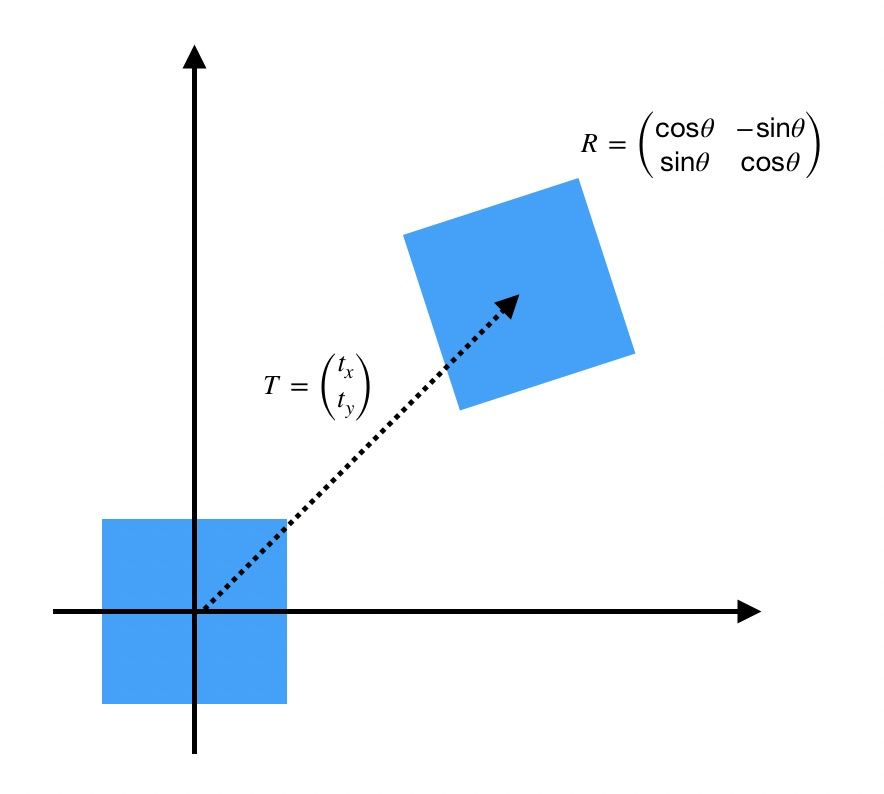
\includegraphics[width=10cm,height=9cm]{rigid body transformation.jpg}
    \caption{rigid body transformation}
\end{figure}

\subsection{Affine Transformation}
\begin{equation}
    \begin{pmatrix}
        x^{\prime} \\ y^{\prime} \\ 1
    \end{pmatrix} = 
    \begin{bmatrix}
        \boldsymbol{A}_{2 \times 2} & \boldsymbol{T}_{2 \times 1}\\
        \boldsymbol{0}^{T} & \boldsymbol{1}
    \end{bmatrix}
    \begin{pmatrix}
        x \\ y \\ 1
    \end{pmatrix}
\end{equation}

\begin{figure}[h]
    \centering
    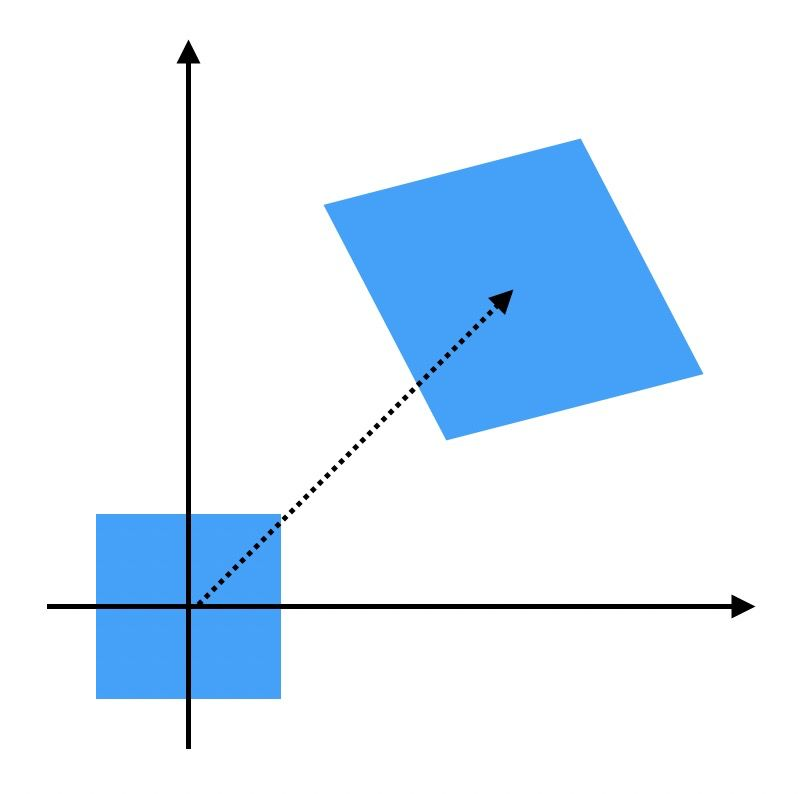
\includegraphics[width=10cm,height=9cm]{affine transformation.jpg}
    \caption{affine transformation}
\end{figure}

\indent where $\boldsymbol{A}_{2\times 2} = 
\begin{bmatrix}
    a_{11} & a_{12} \\
    a_{21} & a_{22}
\end{bmatrix}
$ can be any $2 \times 2 $ matrix, which is different from 
Rigid Body Transformation.\\
\indent Compare with Rigid Body Transformation, Affine Transformation
will not only change the location but also shape of object. However,
transformed object will keep "straightness".

\subsection{Projection Transformation (Homograph Transformation)}
\begin{equation}
    \begin{pmatrix}
        x^{\prime} \\ y^{\prime} \\ 1
    \end{pmatrix} = 
    \begin{bmatrix}
        \boldsymbol{A}_{2 \times 2} & \boldsymbol{T}_{2 \times 1}\\
        \boldsymbol{V}^{T} & \boldsymbol{s}
    \end{bmatrix}
    \begin{pmatrix}
        x \\ y \\ 1
    \end{pmatrix}=
    \boldsymbol{H}_{3\times 3} 
    \begin{pmatrix}
        x \\ y \\ 1
    \end{pmatrix}
\end{equation}

\begin{figure}[h]
    \centering
    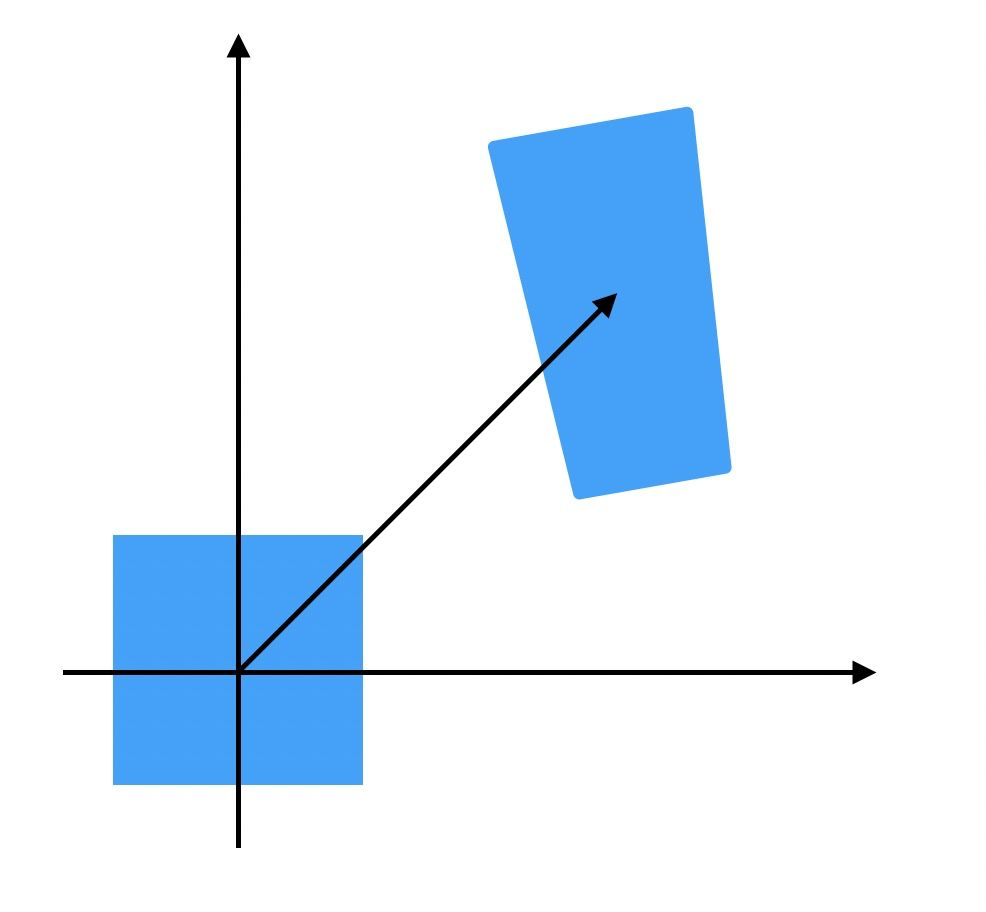
\includegraphics[width=10cm,height=9cm]{homograph transformation.jpg}
    \caption{homograph transformation}
\end{figure}

\indent where $\boldsymbol{A}_{2\times 2}$ is parameters of homograph
transformation, $\boldsymbol{T}_{2\times 1}$ is parameters of
translation transformation. $\boldsymbol{V}^{T} = [v_{1}, v_{2}]$
represents a kind of "edge intersection after transformation" 
relationship and $\boldsymbol{s}$ represents scaling factor related to
$\boldsymbol{V}$ because you will have $v_{1}x+v_{2}y + s = 0$.
Usually, we will make $\boldsymbol{s}=1$ so that,
\begin{equation}
    \begin{bmatrix}
        1 & 0 & 0\\ 0 &1 &0 \\ v_{1} & v_{2} & s
    \end{bmatrix} 
    \begin{pmatrix}
        x \\ y \\ 1
    \end{pmatrix} = 
    \begin{pmatrix}
        x \\ y \\ v_{1}x + v_{2}y + s
    \end{pmatrix}
    \iff
    \begin{pmatrix}
        \frac{x}{v_{1}x + v_{2}y + s} \\
        \frac{y}{v_{1}x + v_{2}y + s}
    \end{pmatrix}
\end{equation}
\indent Here, Homograph Transformation will totally change 
location and shape of object.

\section{Plane coordinate system \& homogeneous coordinate system}
Homogeneous coordinate plane $(x,y,w) \in \mathbb{P}^{3}$ is different
from 3D coordinate system $(x,y,z) \in \mathbb{R}^{3}$, it only has
2 degrees of freedom.
\begin{figure}[h]
    \centering
    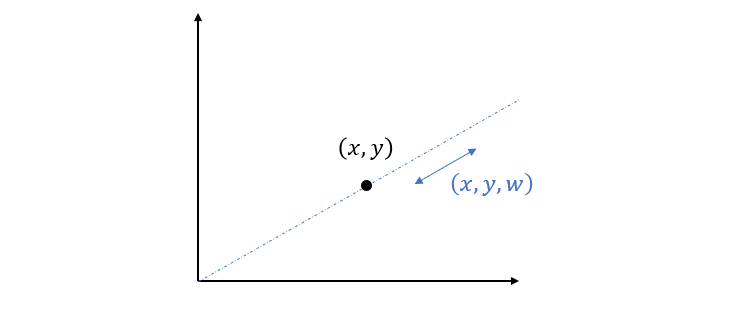
\includegraphics[width=12cm,height=6cm]{coordinate system.png}
    \caption{rotation}
\end{figure}
\begin{equation}
    \begin{pmatrix}
        \frac{x}{w} \\ \frac{y}{w}
    \end{pmatrix}
    \iff\begin{pmatrix}
        x \\ y \\ w
    \end{pmatrix}
\end{equation}
\indent where $w>0$ is scaling factor of $x$ and $y$. When $w=1$,
\begin{equation}
    \begin{pmatrix}
        x \\ y
    \end{pmatrix}
    \iff \begin{pmatrix}
        x \\ y \\ 1
    \end{pmatrix}
\end{equation}
\indent and when $w=0$, it's infinity.
\begin{equation}
    \begin{pmatrix}
        \infty \\ \infty
    \end{pmatrix} \iff
    \begin{pmatrix}
        x\\y\\0
    \end{pmatrix}
\end{equation}
\indent you can clearly see that $(x,y,w)$ slides on the ray
from origin to $(x,y)$.


\section{Homograph Transformation}
Wiki definition: In projective geometry, a homography is an 
isomorphism of projective spaces, induced by an isomorphism 
of the vector spaces from which the projective spaces derive.
mathmatically speaking,

\begin{figure}[h]
    \centering
    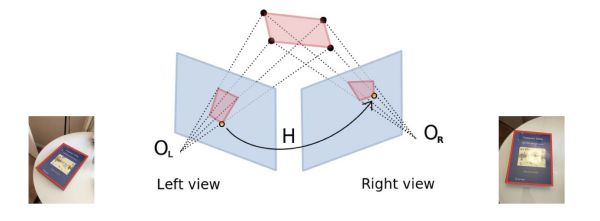
\includegraphics[width=12cm,height=6cm]{homography.jpg}
    \caption{homograph}
\end{figure}

\begin{equation}
    \begin{pmatrix}
        x_{l}\\y_{l}\\1
    \end{pmatrix}=
    \boldsymbol{H}_{3\times 3} \times
    \begin{pmatrix}
        x_{r}\\y_{r}\\1
    \end{pmatrix}
\end{equation}
\indent where $(x_{l},y_{l})$ is the point in one picture and 
$(x_{r}, y_{r})$ is the point in another picture.
For every matching point $(x_{i}, y_{i}) \rightarrow (x_{i}^{\prime},
y_{i}^{\prime})$ we can have,
\begin{equation}
    \begin{pmatrix}
        x_{i}^{\prime} \\ y^{\prime}_{i} \\ 1
    \end{pmatrix} = 
    \begin{bmatrix}
        h_{11} & h_{12} & h_{13}\\
        h_{21} & h_{22} & h{23}\\
        h_{31} & h_{32} & h_{33}
    \end{bmatrix}
    \begin{pmatrix}
        x_{i}\\y_{i}\\1
    \end{pmatrix}=
    \begin{pmatrix}
        h_{11}x_{i} + h_{12}y_{i} + h_{13}\\
        h_{21}x_{i} + h_{22}y_{i} + h_{23}\\
        h_{31}x_{i} + h_{32}y_{i} + h_{33} 
    \end{pmatrix}
\end{equation}
\indent If we translates it to homogeneous coordinate system,
(16) can also be described as,
\begin{align}
    x_{i}^{\prime} &= \frac{h_{11}x_{i} + h_{12}y_{i} + h_{13}}
    {h_{31}x_{i} + h_{32}y_{i} + h_{33}}\\
    y_{i}^{\prime} &= \frac{h_{21}x_{i} + h_{22}y_{i} + h_{23}}
    {h_{31}x_{i} + h_{32}y_{i} + h_{33}}
\end{align}
\indent To see things more clearly, let's write it as form of
$\boldsymbol{A} \boldsymbol{X} = 0$
\begin{equation}
    \begin{bmatrix}
        x_{i} & y_{i} & 1 & 0 & 0 & 0 & -x_{i}^{\prime}x_{i} 
        & -x_{i}^{\prime}y_{i} & x_{i}^{\prime}\\
        0 & 0 & 0 & x_{i} & y_{i} & 1 & -y_{i}^{\prime}x_{i} &
        -y_{i}^{\prime}y_{i} & -y_{i}^{\prime}
    \end{bmatrix}
    \begin{bmatrix}
        h_{11} \\ h_{12} \\h_{13}\\h_{21}\\h_{22}\\h_{23}\\
        h_{31}\\h_{32}\\h_{33}
    \end{bmatrix} = 0
\end{equation}
\indent That's to say, every pair of matching points will have
2 groups of equations.

\subsection{8 degree of freedom}
Here you will notice something interesting, that is homography
matrix $H$ has no difference with $aH$ where $a\neq 0$, because,
\begin{align}
    x_{i}^{\prime} &= \frac{ah_{11}x_{i} + ah_{12}y_{i} + ah_{13}}
    {ah_{31}x_{i} + ah_{32}y_{i} + ah_{33}} = 
    \frac{h_{11}x_{i} + h_{12}y_{i} + h_{13}}
    {h_{31}x_{i} + h_{32}y_{i} + h_{33}}\\
    y_{i}^{\prime} &= \frac{ah_{21}x_{i} + ah_{22}y_{i} + ah_{23}}
    {ah_{31}x_{i} + ah_{32}y_{i} + ah_{33}} =
    \frac{h_{21}x_{i} + h_{22}y_{i} + h_{23}}
    {h_{31}x_{i} + h_{32}y_{i} + h_{33}}
\end{align}
\indent And if we make $a=\frac{1}{h_{33}}$, we can have,
\setlength{\arraycolsep}{3.0pt}
\renewcommand{\arraystretch}{1.5}
\begin{equation}
    \begin{array}{lc}
        \boldsymbol{H}^{\prime} = a\boldsymbol{H} = 
        \begin{bmatrix}
            \frac{h_{11}}{h_{33}} & \frac{h_{12}}{h_{33}} & \frac{h_{13}}{h_{33}}\\
            \frac{h_{21}}{h_{33}} & \frac{h_{22}}{h_{33}} & \frac{h_{23}}{h_{33}}\\
            \frac{h_{31}}{h_{33}} & \frac{h_{32}}{h_{33}} & 1
        \end{bmatrix}
    \end{array}
\end{equation}

\indent here you will only get 8 equations and 8 parameters, hence
if you have 4 pairs of matching points which is nonlinear, you can
have unique solutions.

\section{Python implementation}
\end{document}